% !TeX root = RJwrapper.tex
\title{An overview of R packages for single-source capture-recapture
models}
\author{by Maciej Beręsewicz and Piotr Chlebicki}

\maketitle

\abstract{%
In this paper we provide an overview of R packages that allow fitting
various single-source capture-recapture (SSCR) models. In general, SSCR
approaches assume that capture history follows certain discrete
distribution (e.g.~negative binomial, poisson, one-inflated poisson) but
the observational data consist of only positive counts i.e.~we observe
zero truncated distributions. In this paper we cover both frequentist
and bayesian approach, provide functions for population size estimation
as well as analytical and bootstrap estimators. The paper focus on
\texttt{extraDistr}, \texttt{countreg}, \texttt{VGAM} and \texttt{brms}
packages that are suited for the SSCR models.
}

\hypertarget{introduction}{%
\subsection{Introduction}\label{introduction}}

Introductory section which may include references in parentheses
\citep{R}, or cite a reference such as \citet{R} in the text.

\hypertarget{single-source-capture-recapture-models}{%
\subsection{Single-source capture-recapture
models}\label{single-source-capture-recapture-models}}

\citet{Bohning2022}

\hypertarget{r-package-for-single-source-capture-recapture-model}{%
\subsection{R package for single-source capture-recapture
model}\label{r-package-for-single-source-capture-recapture-model}}

This section may contain a figure such as Figure \ref{fig:Rlogo}.

\begin{Schunk}
\begin{figure}[htbp]

{\centering 
\includegraphics[width=2in]{Rlogo} 

}

\caption[The logo of R]{The logo of R.}\label{fig:Rlogo}
\end{figure}
\end{Schunk}

\hypertarget{truncated-discrete-distributions}{%
\subsubsection{Truncated discrete
distributions}\label{truncated-discrete-distributions}}

In order to use truncated distributions we may use default functions
truncaed at 0

Loading required packages

\begin{Schunk}
\begin{Sinput}
library(extraDistr)
library(countreg)
\end{Sinput}
\begin{Soutput}
#> Loading required package: MASS
\end{Soutput}
\begin{Soutput}
#> Warning: package 'MASS' was built under R version 4.1.2
\end{Soutput}
\begin{Sinput}
library(VGAM)
\end{Sinput}
\begin{Soutput}
#> Warning: package 'VGAM' was built under R version 4.1.2
\end{Soutput}
\begin{Soutput}
#> Loading required package: stats4
\end{Soutput}
\begin{Soutput}
#> Loading required package: splines
\end{Soutput}
\begin{Soutput}
#> 
#> Attaching package: 'VGAM'
\end{Soutput}
\begin{Soutput}
#> The following objects are masked from 'package:countreg':
#> 
#>     dzipois, pzipois, qzipois, rzipois
\end{Soutput}
\begin{Soutput}
#> The following objects are masked from 'package:extraDistr':
#> 
#>     dfrechet, dgev, dgompertz, dgpd, dgumbel, dhuber, dkumar, dlaplace,
#>     dlomax, dpareto, drayleigh, dskellam, dslash, pfrechet, pgev,
#>     pgompertz, pgpd, pgumbel, phuber, pkumar, plaplace, plomax,
#>     ppareto, prayleigh, pslash, qfrechet, qgev, qgompertz, qgpd,
#>     qgumbel, qhuber, qkumar, qlaplace, qlomax, qpareto, qrayleigh,
#>     rfrechet, rgev, rgompertz, rgpd, rgumbel, rhuber, rkumar, rlaplace,
#>     rlomax, rpareto, rrayleigh, rskellam, rslash
\end{Soutput}
\begin{Sinput}
library(brms)
\end{Sinput}
\begin{Soutput}
#> Warning: package 'brms' was built under R version 4.1.2
\end{Soutput}
\begin{Soutput}
#> Loading required package: Rcpp
\end{Soutput}
\begin{Soutput}
#> Warning: package 'Rcpp' was built under R version 4.1.2
\end{Soutput}
\begin{Soutput}
#> Loading 'brms' package (version 2.17.0). Useful instructions
#> can be found by typing help('brms'). A more detailed introduction
#> to the package is available through vignette('brms_overview').
\end{Soutput}
\begin{Soutput}
#> 
#> Attaching package: 'brms'
\end{Soutput}
\begin{Soutput}
#> The following objects are masked from 'package:VGAM':
#> 
#>     acat, cratio, cumulative, dfrechet, dirichlet, exponential,
#>     frechet, geometric, lognormal, multinomial, negbinomial, pfrechet,
#>     qfrechet, rfrechet, s, sratio
\end{Soutput}
\begin{Soutput}
#> The following objects are masked from 'package:extraDistr':
#> 
#>     ddirichlet, dfrechet, pfrechet, qfrechet, rdirichlet, rfrechet
\end{Soutput}
\begin{Soutput}
#> The following object is masked from 'package:stats':
#> 
#>     ar
\end{Soutput}
\begin{Sinput}
library(numDeriv)
\end{Sinput}
\end{Schunk}

\hypertarget{extradistr}{%
\subsubsection{extraDistr}\label{extradistr}}

\begin{Schunk}
\begin{Sinput}
library(extraDistr)
set.seed(123)
\end{Sinput}
\end{Schunk}

\hypertarget{countreg}{%
\subsubsection{countreg}\label{countreg}}

\texttt{countreg} package includes function \texttt{zerotrunc}

\hypertarget{vgam}{%
\subsubsection{VGAM}\label{vgam}}

The most advanced

\hypertarget{stan-and-brms}{%
\subsubsection{stan and brms}\label{stan-and-brms}}

\hypertarget{case-studies}{%
\subsection{Case studies}\label{case-studies}}

There will likely be several sections, perhaps including code snippets,
such as:

\begin{Schunk}
\begin{Sinput}
x <- 1:10
plot(x)
\end{Sinput}

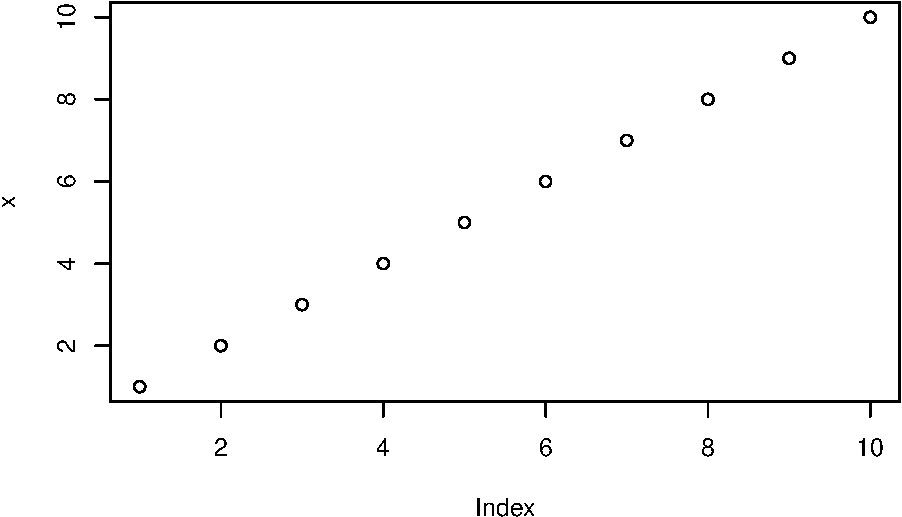
\includegraphics{overview-single-source_files/figure-latex/unnamed-chunk-3-1} \end{Schunk}

\hypertarget{summary}{%
\subsection{Summary}\label{summary}}

This file is only a basic article template. For full details of
\emph{The R Journal} style and information on how to prepare your
article for submission, see the
\href{https://journal.r-project.org/share/author-guide.pdf}{Instructions
for Authors}.

\hypertarget{acknowledgement}{%
\subsection{Acknowledgement}\label{acknowledgement}}

This work was financially supported by the NCN OPUS 22 grant no.
2020/39/B/HS4/00941.

\bibliography{overview-single-source.bib}

\address{%
Maciej Beręsewicz\\
Poznań University of Economics and Business\\%
Al. Niepodległości 10\\ 61-875 Poznań, Poland\\
Statistical Office in Poznań\\%
ul. Wojska Polskiego 27/29\\ 60-624 Poznań, Poland\\
%
\url{https://ncn-foreigners.github.io/}\\%
\textit{ORCiD: \href{https://orcid.org/0000-0002-8281-4301}{0000-0002-8281-4301}}\\%
\href{mailto:maciej.beresewicz@ue.poznan.pl}{\nolinkurl{maciej.beresewicz@ue.poznan.pl}}%
}

\address{%
Piotr Chlebicki\\
Adam Mickiewicz University\\%
ul. Wieniawskiego 1\\ 61-712 Poznań, Poland\\
%
\url{https://github.com/Kertoo}\\%
%
\href{mailto:piochl@st.amu.edu.pl}{\nolinkurl{piochl@st.amu.edu.pl}}%
}
